\documentclass{article}

\usepackage[left=2cm,right=2cm, top=2cm, bottom = 2cm]{geometry}
\usepackage{amsfonts}

\usepackage{amsmath}
\usepackage{xcolor}

\usepackage{tikz}
\usepackage{subfigure}



\pagestyle{empty}

\setlength{\tabcolsep}{15pt}


\newcommand{\deriv}[3][]{\frac{\mathrm{d}^{#1}#2}{\mathrm{d}#3^{#1}}}
\newcommand{\diff}{\;\mathrm{d}}

\newcommand{\norm}[1]{\left|\kern-1pt\left|#1\right|\kern-1pt\right|}
\newcommand{\bra}[1]{\left\langle #1 \,\right|}
\newcommand{\ket}[1]{\left|\, #1\right\rangle}
\newcommand{\braket}[2]{\left\langle #1 \mid #2 \right\rangle}




\begin{document}

\title{Root Locus Diagrams}
\date{}

\maketitle
\thispagestyle{empty}

\Large

\vskip -10mm

\textbf{\underline{Objective: To draw and interpret root locus diagrams.}}








\vspace{5mm}






\textbf{Warm-Up: Proportional Control:}\bigskip

Suppose we have a system with open-loop transfer function $\frac{1}{s(s+3)}$. This is type 1 (it has an integrator---a factor of $\frac{1}{s}$---in the forward path), so it will have 0 steady-state error for a step input. However, we also care about the response time to the step input, and any potential overshoot. To attempt to control these, we introduce a proportional controller, which simply amplifies the error by some constant gain $K$ before feeding through the open loop:
\begin{center}
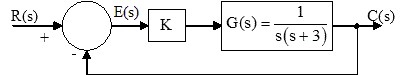
\includegraphics{P-control.jpg}
\end{center}

The closed-loop transfer function of this system is
\[\frac{K\frac{1}{s(s+3)}}{1+K\frac{1}{s(s+3)}}=\frac{K}{s^2+3s+K},\]
so to understand this system (by, for instance, a partial fractions decomposition) we wish to factorise $s^2+3s+K$, for which we need to know the roots. In order to choose a value of $K$ which will meet our requirements for the system, therefore, we wish to study how the roots of $s^2+3s+K$ vary as $K$ varies.

\begin{enumerate}
	\item Show that the roots of the denominator are given by
		\[s=-\frac{3}{2}\pm \frac{1}{2}\sqrt{9-4K}.\]
	\item Plot the two roots on an Argand diagram for $K=1,2,3,10,20$.
	\item Describe the behaviour you would expect from the system for each of the above values of $K$.
	\item Find the value of $K$ at which critical damping occurs.
\end{enumerate}


\clearpage






\textbf{Theory: Root Locus Diagrams:}\bigskip

A large part of the analysis of a system depends on studying the locations of its poles, which are the roots of its denominator. A \textbf{root locus diagram} shows how the roots of a function vary as some parameter of the system varies. For instance, in the warm-up we studied how the roots of $s^2+3s+K$ vary as the gain of the proportional controller $K$ was varied.

Suppose we have a system with open-loop transfer function $KG(s)$, where $K$ is a constant parameter under our control; this will be the case for a proportional control system. The closed-loop transfer function with unity-gain negative feedback is then
\[\frac{KG(s)}{1+KG(s)}.\]
This will have poles where $KG(s)=-1$, so we are interested in studying solutions of $KG(s)=-1$ and how they depend on $K$. As we did when looking at Bode plots, we split the condition $KG(s)=-1$ into two: $|KG(s)|=1$ and $\arg(KG(s))=(2n+1)180^\circ$, where $n$ is any integer. So for each value of $K$ we want to find the values of $s$ which make $|KG(s)|=1$ and $\arg(KG(s))=(2n+1)180^\circ$.

If $G(s)$ is a rational function with real coefficients (which it will be for a system with no delay), then we can write $G(s)=\frac{N(s)}{D(s)}$, for some numerator and denominator polynomials $N(s)$ and $D(s)$ respectively. Then $KG(s)=-1$ if and only if $KN(s)=-D(s)$, which is a polynomial equation with real coefficients, so its solutions occur in complex conjugate pairs. Therefore the root locus will be symmetrical in the real axis.\medskip

Below is the root locus for the transfer function
\[G(s)=\frac{s^2+2s+2}{s(s^4+9s^3+33s^2+51s+26)}.\]


\begin{center}
	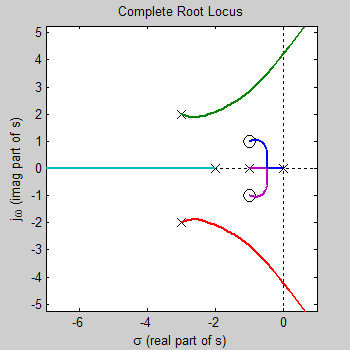
\includegraphics[scale=0.5]{RLTotal.png}
\end{center}

\clearpage











\textbf{Theory: Sketching the Root Locus:}\bigskip

Computational packages such as MatLab have built-in functions for plotting root loci. There are also a number of techniques allowing you to sketch a root locus from knowledge of the open-loop transfer function.

From the modulus condition, $|KG(s)|=1$, we see that as $K\to 0$, we must have $|G(s)|\to\infty$; so the first step in plotting a root locus is to find the poles of $G(s)$, and mark these with crosses; they are the points from which the branches of the root locus start.

Similarly, as $K\to\infty$, to maintain $|KG(s)|=1$, we must have $G(s)\to 0$. There are two ways in which $G(s)+\frac{N(s)}{D(s)}$ can tend to 0; either as $s$ tends to a root of the numerator $N(s)$, or as $|s|\to \infty$ (assuming that the degree of $D$ is strictly greater than the degree of $N$).

So each branch of the root locus starts at a pole of $G(s)$ and tends either to infinity or to a root of $G(s)$.\medskip

Consider the argument condition: $\arg(KG(s))=(2n+1)180^\circ$; if we factor $N(s)$ as $(s-z_1)\hdots(s-z_k)$ and $D(s)$ as $(s-p_1)\hdots(s-p_m)$, then
\[\arg(KG(s))=\sum_{i=1}^k \arg(s-z_i) - \sum_{i=1}^m \arg(s-p_i).\]
If $z_1$ and $z_2$, say, are a complex conjugate pair, then $\arg(s-z_1)+\arg(s-z_2)=0$ (draw a picture!), and similarly for poles $p_i$; so complex zeros and poles cancel out and make no contribution to the argument. Therefore we can consider only poles and zeros on the real axis. Then $\arg(s-z_i)$ (or $\arg(s-p_i)$) is $180^\circ$ if $s$ is to the right of $z_i$ and is 0 otherwise. So for $s$ on the real axis, we can only get $\arg(KG(s))=(2n+1)180^\circ$ if the number of real zeros of $G$ to the right of $s$, minus the number of real poles of $G$ to the right of $s$, is an odd number. This constrains the parts of the real axis that can lie on our root locus, and will tell us which direction a branch starting on the real axis must go in.\medskip



There are a number of other rules for sketching root loci; see \begin{verbatim}https://lpsa.swarthmore.edu/Root_Locus/DeriveRootLocusRules.html\end{verbatim} for more!


\end{document}